\documentclass[midd]{thesis}

\usepackage{graphicx}
\usepackage{times}

\bibliographystyle{plain}

\title {Hybrid Computational Aesthetic Evaluation using Convolutional Neural Networks: Filtering Generative Art through Interactive Modeling of User Tastes}

\author {Teddy Knox}
\adviser {Professor Christopher Andrews}

\begin{document}

\maketitle

\begin{abstract}
Recent advances in machine learning techniques have resulted in increasingly effective algorithms for discovering creative
solutions to quantifiable optimization problems. In general, problems unaffected by advances in machine learning are not
those involving creativity, but those whose optimization functions are difficult to quantify. To teach a computer to
produce aesthetically pleasing artwork, one first must define a \"cost\" function for what makes a piece aesthetically
pleasing, either manually or automatically. We're going to try to use Convolutional Neural Networks to make a hybrid
Computational Aesthetic Evaluation function and generate artwork that appeals to the user.
\end{abstract}

\begin{acknowledgements}
I dedicate this paper to science.
\end{acknowledgements}

\contentspage
\tablelistpage
\figurelistpage

\normalspacing \setcounter{page}{1} \pagenumbering{arabic}

\chapter{Introduction}
\label{sec:intro}

\chapter{Related Work}

\section{Related Work in Generative Art}

\section{Related Work in Generative Art}

\chapter{Theory}

\section{Generative Art}

\section{CAE-CNN}

\chapter{Implementation}

\section{Generative Art}

\section{CAE-CNN}

\chapter{Results}

Quantitative results here

\chapter{Conclusion}

Qualitative results here

% \chapter{Bibliography}
\bibliographystyle{plain}
\bibliography{thesis}
\cite{takagi, galanter-1, galanter-2, galanter-3}

% This thesis has many chapters.  For more on Alice see
% Chapter~\ref{sec:alice}, and in particular Section~\ref{sec:reproach}.
%
% \section{SECTION 1}
% The text for Section 1 goes here.
%
% \section{SECTION 2}
% Section 2 text.
%
% \subsection{Subsection heading goes here}
% Subsection 1 text
%
% \subsubsection{Subsubsection 1 heading goes here}
% Subsubsection 1 text
%
% \subsubsection{Subsubsection 2 heading goes here}
% Subsubsection 2 text
%
% \section{SECTION 3}
% Section 3 text. The dielectric constant at the air-metal interface
% determines the resonance shift as absorption or capture occurs.
%
% \begin{equation}
% \label{eqn:sampleEqn}
% k_1=\frac{\omega }{c({1/\varepsilon_m + 1/\varepsilon_i})^{1/2}}=k_2=\frac{\omega
% sin(\theta)\varepsilon_{air}^{1/2}}{c}
% \end{equation}
%
% \noindent
% where $\omega$ is the frequency of the plasmon, $c$ is the speed of
% light, $\varepsilon_m$ is the dielectric constant of the metal,
% $\varepsilon_i$ is the dielectric constant of neighboring insulator,
% and $\varepsilon_{air}$ is the dielectric constant of air.
% Equation~\ref{eqn:sampleEqn} makes this perfectly clear.
% See also Figure~\ref{fig:myfig} for an illustration.
%
%
% \begin{figure}
% \centering
% 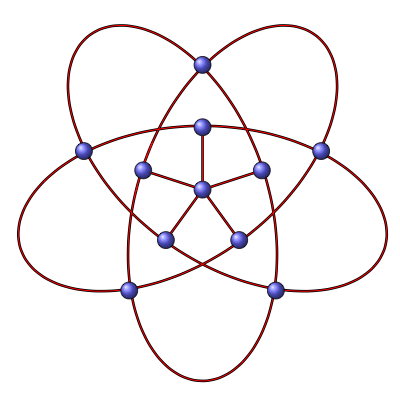
\includegraphics[width=0.75\textwidth]{graph.png}
% \caption{My figure.}
% \label{fig:myfig}
% \end{figure}
%
% \chapter{Alice in Wonderland}
% \label{sec:alice}
%
% \section{The Black Kitten}
%   One thing was certain, that the WHITE kitten had had nothing to
% do with it:---it was the black kitten's fault entirely~\cite{aiw}.  For the
% white kitten had been having its face washed by the old cat for
% the last quarter of an hour (and bearing it pretty well,
% considering); so you see that it COULDN'T have had any hand in
% the mischief.
%
%   The way Dinah washed her children's faces was this:  first she
% held the poor thing down by its ear with one paw, and then with
% the other paw she rubbed its face all over, the wrong way,
% beginning at the nose:  and just now, as I said, she was hard at
% work on the white kitten, which was lying quite still and trying
% to purr---no doubt feeling that it was all meant for its good.
%
%   But the black kitten had been finished with earlier in the
% afternoon, and so, while Alice was sitting curled up in a corner
% of the great arm-chair, half talking to herself and half asleep,
% the kitten had been having a grand game of romps with the ball of
% worsted Alice had been trying to wind up, and had been rolling it
% up and down till it had all come undone again; and there it was,
% spread over the hearth-rug, all knots and tangles, with the
% kitten running after its own tail in the middle.
%
% \section{The Reproach}
% \label{sec:reproach}
%
% (As promised in Chapter~\ref{sec:intro}, here it gets interesting.)
%
%   `Oh, you wicked little thing!' cried Alice, catching up the
% kitten, and giving it a little kiss to make it understand that it
% was in disgrace.  `Really, Dinah ought to have taught you better
% manners!  You OUGHT, Dinah, you know you ought!' she added,
% looking reproachfully at the old cat, and speaking in as cross a
% voice as she could manage---and then she scrambled back into the
% arm-chair, taking the kitten and the worsted with her, and began
% winding up the ball again.  But she didn't get on very fast, as
% she was talking all the time, sometimes to the kitten, and
% sometimes to herself.  Kitty sat very demurely on her knee,
% pretending to watch the progress of the winding, and now and then
% putting out one paw and gently touching the ball, as if it would
% be glad to help, if it might.
%
%   `Do you know what to-morrow is, Kitty?' Alice began.  `You'd
% have guessed if you'd been up in the window with me---only Dinah
% was making you tidy, so you couldn't.  I was watching the boys
% getting in stick for the bonfire---and it wants plenty of
% sticks, Kitty!  Only it got so cold, and it snowed so, they had
% to leave off.  Never mind, Kitty, we'll go and see the bonfire
% to-morrow.'  Here Alice wound two or three turns of the worsted
% round the kitten's neck, just to see how it would look:  this led
% to a scramble, in which the ball rolled down upon the floor, and
% yards and yards of it got unwound again.
%
%   `Do you know, I was so angry, Kitty,' Alice went on as soon as
% they were comfortably settled again, `when I saw all the mischief
% you had been doing, I was very nearly opening the window, and
% putting you out into the snow!  And you'd have deserved it, you
% little mischievous darling!  What have you got to say for
% yourself?  Now don't interrupt me!' she went on, holding up one
% finger.  `I'm going to tell you all your faults.  Number one:
% you squeaked twice while Dinah was washing your face this
% morning.  Now you can't deny it, Kitty:  I heard you!  What that
% you say?' (pretending that the kitten was speaking.)  `Her paw
% went into your eye?  Well, that's YOUR fault, for keeping your
% eyes open---if you'd shut them tight up, it wouldn't have
% happened.  Now don't make any more excuses, but listen!  Number
% two:  you pulled Snowdrop away by the tail just as I had put down
% the saucer of milk before her!  What, you were thirsty, were you?
%
% \chapter{Chapter 3}
%
% \chapter{Chapter 4}
%
% \appendix
% \chapter{Chapter 1 of appendix}
% Appendix chapter 1 text goes here

\end{document}
